% !TEX root = ../../main.tex


\begin{figure}[!htb]
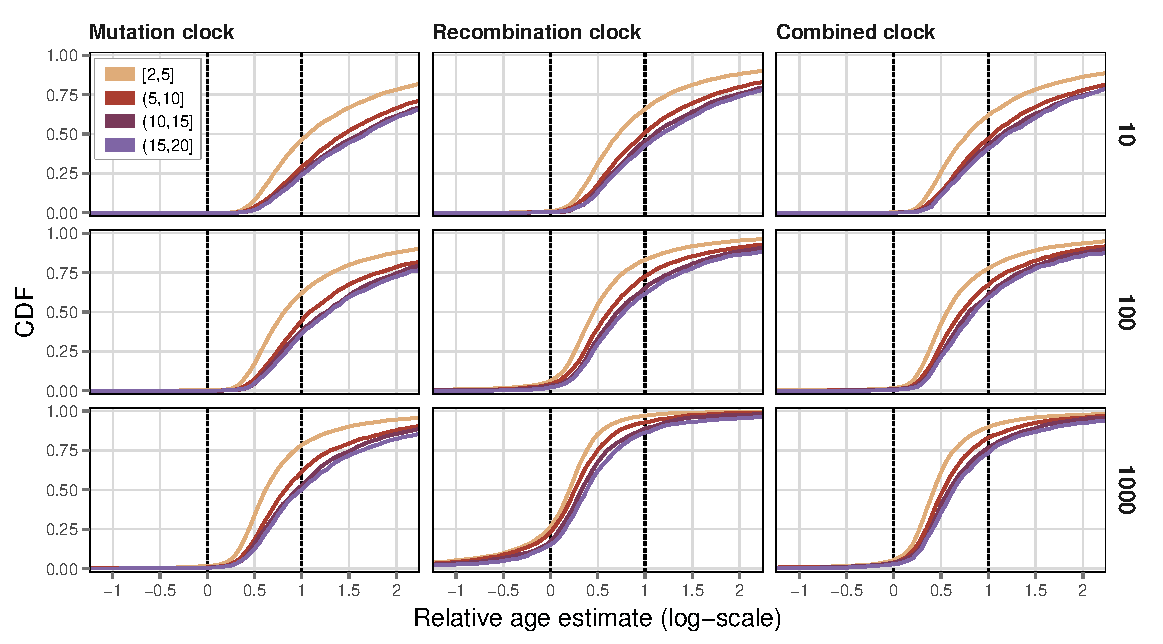
\includegraphics[width=\textwidth]{./img/ch5/discords_hist}
\Caption{Relative age under varying numbers of discordant pairs}
{A randomly drawn set of \n{10000} target sites at allele frequency ${\leq 1\%}$, \ie \fk{[2,20]}, was analysed under each of the \n{3} clock models (indicated at the \emph{top} of each column) and with different numbers of sampled discordant pairs; ${n_d = \num{10}}$, ${n_d = \num{100}}$, and ${n_d = \num{1000}}$ (indicated at the \emph{right} of each row).
The analysis was conducted using the true IBD breakpoints as derived from simulation records, defined as the first variant sites observed in the data that immediately follow the \n{2} recombination events on each side distal to a given focal site.
The relative age, ${\hat{t}_\textit{rel}}$, was calculated as given in \cref{eq:age_relative}, such that the true times of concordant and discordant coalescent events, $t_c$ and $t_d$, sit at 0~and~1, respectively (\emph{dashed} lines).
Note that ${\hat{t}_\textit{rel}}$ is defined on log-scale.
The \gls{cdf} of relative age estimates is shown per \fk{}~group, where target variants were pooled by their allele count in the data, in ranges of \fk{[2,5]}, \fk{(5,10]}, \fk{(10,15]}, and \fk{(15,20]}.}
{fig:discords_hist}
\end{figure}
